%%%%%%%%%%%%%%%%%%%%%%%%%%%%%%%%%%%%%%%%%%%%%%%%%%%%%%%%%%%%%%%%%%%%%%%%%%%%%%%%%%%%%%%%%%%%%%%%%%%%%%%%%%%%%%%%%%%%%%%%%%
% Project 6: Modeling and simulation of flash LiDAR detection systems
%%%%%%%%%%%%%%%%%%%%%%%%%%%%%%%%%%%%%%%%%%%%%%%%%%%%%%%%%%%%%%%%%%%%%%%%%%%%%%%%%%%%%%%%%%%%%%%%%%%%%%%%%%%%%%%%%%%%%%%%%%
\documentclass[../../me144_244_student.tex]{subfiles}
\begin{document}
\pagestyle{mypagestyle}
\project{6}{Modeling and simulation of flash LiDAR systems (100 points)}{November 3rd, 2026 @ 11:59PM PST}[Add instructions]

\subsection*{Introduction}

As discussed in lecture, LiDAR (Light Detection and Ranging) systems are highly
effective at capturing a 3D representation of surfaces for the purposes of mapping or inspecting
geometry. When deployed using a drone, this can be done quickly, safely, and autonomously,
enabling applications such as the continuous inspection of infrastructure to detect damage
before more catastrophic failure can occur. However, as we will see in this assignment, there are
potentially many design decisions that can impact the effectiveness of a LiDAR system when deployed.
Therefore, our goal is to develop a fast simulation that could be used in an optimization
study where it may have to be run hundreds or thousands of times.

\subsection*{Surface Model}

We would like to be able to evaluate our LiDAR system on test surfaces to get an
idea of how well it will perform on real objects, which vary greatly in geometry. In this project
we will use a mathematically designed surface, given by the implicit function representation:

\vspace{0.1 in}
\begin{equation}\label{surfG}
    G(x_1, x_2, A) = 2 + A \sin\bigg(\frac{2 \omega_1 \pi x_1}{L_1}\bigg) \sin\bigg(\frac{2 \omega_2 \pi x_2}{L_2}\bigg)
\end{equation}
\vspace{0.1 in}

where $A$ is a defined constant that parameterizes the function. As $A$ varies, the angles of the
surface changes the direction of reflection for each of the rays, and thus may increase or decrease
the rays that undergo multiple reflections. This essentially gives us axis that allows us to control
how smooth the test surface is, indicating the system's performance on smooth or rough objects.
The surface is centered about the height $x_3 = 2$\,m, about 1\,m below the scanner, which sits at
$z_0 = 3$\,m.

\subsubsection*{Surface normal}

To model the reflection of a ray we need the surface normal $\boldsymbol{n}_i$ precisely at the
location in which the ray comes into contact with the surface. Recall from multi-variable calculus
that the surface normal and components of the gradient can be computed as:

\vspace{0.1 in}
\begin{equation}
    \boldsymbol{n}_i = \frac{\nabla F}{||\nabla F||_2}
\end{equation}

\begin{equation}
    \nabla F = \frac{\partial F}{\partial x_1} \boldsymbol{e}_1 + \frac{\partial F}{\partial x_2} \boldsymbol{e}_2 + \frac{\partial F}{\partial x_3}\boldsymbol{e}_3.
\end{equation}
\vspace{0.1 in}

It is beneficial to rewrite the surface function $G(x_1, x_2)$ in parametric form when computing the
gradient:

\vspace{0.1in}
\begin{equation}
    F(x_1, x_2, x_3) = G(x_1, x_2) - x_3 = 0
\end{equation}
\vspace{0.2in}
The gradient can be rewritten as:

\vspace{0.1 in}
\begin{equation}\label{gradF}
    \nabla F = \frac{\partial G}{\partial x_1} \boldsymbol{e}_1 + \frac{\partial G}{\partial x_2} \boldsymbol{e}_2 - \boldsymbol{e}_3
\end{equation}
\vspace{0.1in}

With this choice of $F$, the normal points down, into the surface: a ray travelling toward the
surface satisfies $\boldsymbol{v}_i \cdot \boldsymbol{n}_i > 0$.

\subsection*{Model Formulation}

We will use a discrete ray model to simulate the light emitted from a single pulse of a flash LiDAR
system. We track many rays which leave the emitter with a given direction, tracking them as they
propagate through space, intersect with the test surface, and ultimately hit or miss the sensor on
their return. The following subsections follow the path of the light: the optics that define the
field of view, the emission of the rays, their propagation and reflection from the surface, their
detection by the receiver, and finally the reconstruction of the surface from the measured times.

\subsubsection*{Optics}
In practice, LiDAR systems require \textbf{optics} which are necessary to re-size the area being
scanned to the size of the sensor element, otherwise sensors would have to be impractically large
instead of small, centimeter scale devices. In our simulation, our optics will comprise a thin
(ideal) lens and an aperture, which limits how much light can enter the lens. You will be provided
the lens model in the starter code along with a detailed description of how it works for your
reference.

The lens is characterized by its focal length $f$, the distance $d_f$ to the plane that is in focus
(set to the distance to the surface), and the radius $a$ of the aperture. The thin lens equation,
$\frac{1}{f} = \frac{1}{d_f} + \frac{1}{s'}$, gives the distance $s'$ from the lens to the focal
plane array of $n_{\text{pix}} \times n_{\text{pix}}$ pixels of size $p$, so that light from the
in-focus plane is brought to a single point on the array. As seen in Figure~\ref{fig:flash}, the
lens then allows the small sensor to `see' a comparatively large area, the field of view (FOV), whose
half angle follows from the size of the array,
\begin{equation}
    \tan\theta_{\text{FOV}} = \frac{n_{\text{pix}}\, p}{2 s'}.
\end{equation}
Lengthening the focal length increases $s'$ and so narrows the field of view. Since this is the
maximum extent we can map, our emitter only casts light over the FOV. You will investigate how
changing the FOV impacts the quality of reconstruction.

\begin{figure}[H]
    \centering
    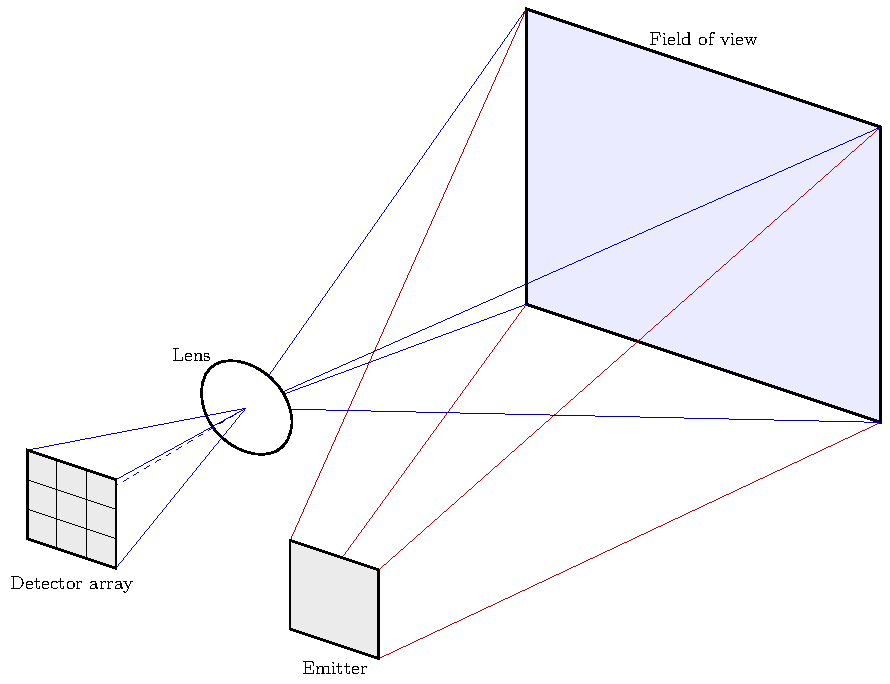
\includegraphics[width=0.7\linewidth]{fig_flash_lidar.pdf}
    \caption{Flash LiDAR. The sensor's FOV determines how large of an area can be reconstructed.}
    \label{fig:flash}
\end{figure}

\subsubsection*{Ray emission}
The emitter is idealized as a point source located at the center of the lens, $\boldsymbol{r}_0 =
(0, 0, z_0)$, which sends $N$ rays downward toward the surface, each with speed $c$. The starter code
provides the initial ray directions: the slopes $t_x, t_y$ are drawn uniformly over the field of view
and give the unit direction $\hat{\boldsymbol{d}}_0$ of each ray,
\begin{equation}
    t_x, t_y \sim \mathcal{U}\big(-\tan\theta_{\text{FOV}},\, \tan\theta_{\text{FOV}}\big), \qquad
    \hat{\boldsymbol{d}}_0 = \frac{(t_x, t_y, -1)}{\|(t_x, t_y, -1)\|_2}.
\end{equation}
You are responsible for placing every ray at the emitter and giving it the initial velocity
$\boldsymbol{v}_i(0) = c\,\hat{\boldsymbol{d}}_0$.

\subsubsection*{Propagation and reflection}
Each ray travels in a straight line between interactions with the surface, so we advance the ray
positions in time with the Forward Euler method,
\begin{equation}
    \boldsymbol{r}_i(t + \Delta t) = \boldsymbol{r}_i(t) + \Delta t\, \boldsymbol{v}_i(t).
\end{equation}
After every step, a ray has reached the surface if it is at or below it, $x_{3,i} \le G(x_{1,i}, x_{2,i})$.

When a ray reaches the surface (Figure~\ref{fig:raypath}), we model its interaction using the classical
law of reflection: the angle of incidence equals the angle of reflection. For a specular surface we
also assume for simplicity that:

\begin{itemize}
    \item the features of the surface are at least an order of magnitude larger than the wavelength of
    the incident radiation, so that ``geometric'' ray tracing theory is applicable,
    \item and the reflectance parameter $I\!\!R = 1$ (no absorption).
\end{itemize}

The velocity of the ray immediately after reflection, $\boldsymbol{v}_i^{ref}$, is found by first
projecting the incoming velocity $\boldsymbol{v}_i$ onto the surface normal $\boldsymbol{n}_i$ to
obtain its normal component:
\begin{equation}
    \boldsymbol{v}_i^\perp = \frac{\boldsymbol{v}_i \cdot \boldsymbol{n}_i}{\boldsymbol{n}_i \cdot \boldsymbol{n}_i} \boldsymbol{n}_i .
\end{equation}
Subtracting this normal component twice flips the sign of the normal component of the outgoing ray
while leaving the tangential component unchanged:
\begin{equation}\label{vref}
    \boldsymbol{v}_i^{ref} = \boldsymbol{v}_i - 2\boldsymbol{v}_i^{\perp}.
\end{equation}

\begin{figure}[H]
    \centering
    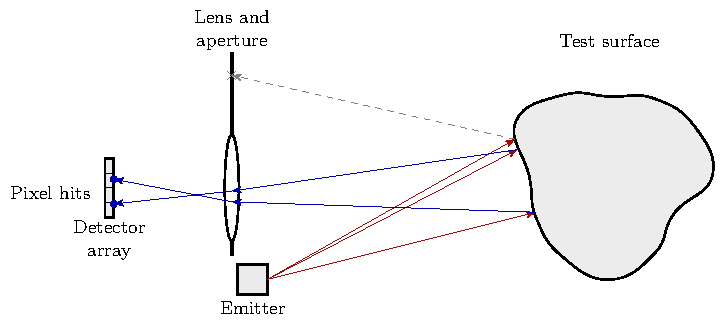
\includegraphics[width=0.5\linewidth]{fig_ray_path.pdf}
    \caption{Ray paths in a side view. Rays emitted from the source (red) reflect off the test surface according to the law of reflection. Returning rays (blue) that pass through the lens aperture are focused onto a detector pixel; a ray whose return misses the aperture (gray dashed) is never detected.}
    \label{fig:raypath}
\end{figure}

Because the time step has a finite size, a ray will usually overshoot the surface slightly, and may
even still be below the surface after it reflects. We therefore only reflect a ray if it is moving
\emph{into} the surface, $\boldsymbol{v}_i \cdot \boldsymbol{n}_i > 0$. Without this check, a ray that
is still below the surface after reflecting would be reflected a second time and sent back into the
surface.

We have also provided a model for diffuse (Lambertian) reflection, which is the reflection law
characteristic of ``matte'' materials. Under Lambertian reflection, the reflected intensity per unit
area is the same from all viewing angles. Each reflection in the starter code is diffuse with
probability \texttt{diffuseFraction} and specular otherwise, so \texttt{diffuseFraction}\,$=0$ is a
pure mirror and \texttt{diffuseFraction}\,$=1$ (the default) is a purely matte surface. You will
investigate how varying the surface appearance between specular and diffuse impacts the quality of
reconstruction.

A ray can reflect several times from a non-convex surface. Rays that reflect more than
\texttt{maxBounces} times are discarded, as are rays that leave the sensor range, $|x_1|$ or $|x_2| >
\texttt{domainMax}$.

\subsubsection*{Detection}
The receiver sits in the plane $z = z_0$. A ray is detected when, after a time step, it has crossed this
plane going upward ($x_3 > z_0$) \emph{and} the crossing point lies inside the aperture,
$x_1^2 + x_2^2 \le a^2$. Rays that cross the plane outside the aperture are lost, and a ray that has
crossed the plane is no longer tracked. Since the ray overshoots the plane during the final time step,
the crossing time is
\begin{equation}
    t_{j,i} = t - \frac{x_{3,i} - z_0}{v_{3,i}},
\end{equation}
where $t$ is the current time. The starter code takes each detected ray through the lens to the pixel
it lands on, and registers the time it would have taken a ray through the lens center. Each pixel keeps
only its first return, $t_{\text{pix}}$.

\subsubsection*{Time of flight and reconstruction}
Flash LiDAR works according to the time-of-flight principle. By tracking the time elapsed between
emitting and detecting a pulse of light, we can determine the length of the path the light travelled
using the speed of light. We model the emitter as being located at the center of the lens; in
practice this assumption holds as the distance between emitter and detector is small relative to the
distance to the object. Thus, the light travels the same distance going out as it does on its return,
and the distance from the lens to the surface point seen by a pixel is
\begin{equation}
    R = \frac{c\, t_{\text{pix}}}{2}.
\end{equation}
However, this distance is meaningless unless we know at which point the light intersected the surface.
The benefit of using optics is that (when the subject is in focus) the lens redirects all light
originating from a single surface point to a single point on the sensor. Thus, by tracing a ray in
reverse, we can locate where the light hitting a given pixel originated from. As seen in
Figure~\ref{fig:chief}, the chief ray of a sensor pixel points from the pixel center through the
center of the lens. The reconstructed surface point is therefore found by travelling a distance $R$
from the emitter along the chief ray,
\begin{equation}
    \boldsymbol{r}_p = \boldsymbol{r}_0 + R\, \hat{\boldsymbol{d}}_{\text{pix}},
\end{equation}
where $\hat{\boldsymbol{d}}_{\text{pix}}$ is the unit vector along the chief ray of the pixel (provided
in the starter code). Pixels with no return produce no point. Since the position of the sensor
relative to some reference point is generally known, we can accumulate all of the points into a
grounded 3D representation.

\begin{figure}[H]
    \centering
    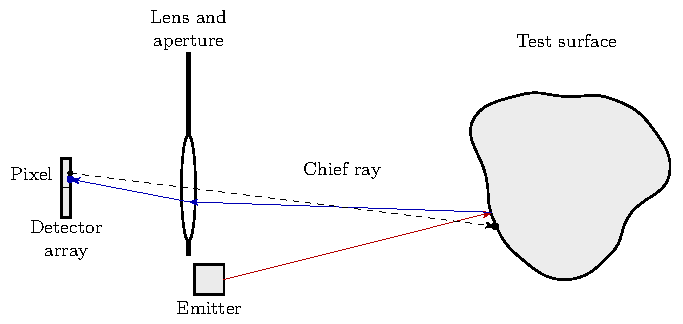
\includegraphics[width=0.7\linewidth]{fig_chief_ray.pdf}
    \caption{Chief ray of a pixel. A ray returning from the surface (blue) strikes the pixel off-center, but all light landing on the pixel is assigned to its chief ray (dashed), which passes from the pixel center through the center of the lens. The surface point is placed along the chief ray at the distance $R$ given by the time of flight.}
    \label{fig:chief}
\end{figure}

\subsubsection*{Reconstruction error}
We measure the quality of a reconstruction in two ways. The \textbf{error} is the fraction of pixels that
received no return,
\begin{equation}
    \text{ERROR} = \frac{\text{PIXELS WITHOUT A RETURN}}{n_{\text{pix}}^2}.
\end{equation}
This measures \emph{coverage} only. To judge the \emph{accuracy} of the pixels that do have a return, each
pixel's reconstructed height is compared to the true height of the surface, averaged over that pixel's
footprint on the surface (the area it sees). A pixel sees a patch of surface rather than a single point,
so this mean height is the quantity that the pixel can be expected to recover. These comparisons are
computed for you by \texttt{reference.py}, which you should not edit.

\vspace{1 em}
\centerline{ \bf VARIABLE GLOSSARY}
\vspace{.1 in}

\begin{table}[H]
  \begin{center}
  \caption{Simulation parameters (defaults in the starter code)}
  \begin{tabular}{||c|c|c|c|l||}
    \hline
    Symbol & Code name & Units & Value & Description \\
    \hline \hline
    $A$ & \texttt{A\_} & m & [0.04, 0.16, 0.64] & Surface amplitudes \\
    $L_1, L_2$ & \texttt{L1, L2} & m & 1 & Surface oscillation lengths \\
    $\omega_1, \omega_2$ & \texttt{omega1, omega2} & -- & 2, 1 & Surface frequencies \\
    $c$ & \texttt{c} & m/s & $3 \times 10^8$ & Speed of light \\
    $z_0$ & \texttt{z0} & m & 3 & Scanner (lens and emitter) height \\
    $N$ & \texttt{nRays} & -- & 200,000 & Number of rays \\
    $\Delta t$ & \texttt{dt} & s & $0.001\, z_0 / c$ & Time step \\
    -- & \texttt{domainMax} & m & 5 & Rays leaving $|x_1|, |x_2| >$ this are lost \\
    -- & \texttt{maxBounces} & -- & 10 & Rays reflecting more times are lost \\
    -- & \texttt{diffuseFraction} & -- & 1 & Fraction of reflections that are diffuse \\
    $f$ & \texttt{f} & m & 0.1 (and 0.2) & Lens focal length \\
    $d_f$ & \texttt{focusDist} & m & 1 & Distance from the lens to the plane in focus \\
    $s'$ & \texttt{sensorDist} & m & from thin lens eqn. & Lens to focal plane array distance \\
    $a$ & \texttt{apertureRadius} & m & 0.1 & Lens aperture radius \\
    $p$ & \texttt{pixelPitch} & m & $4 \times 10^{-3}$ & Pixel size \\
    $n_{\text{pix}}$ & \texttt{nPix} & -- & 32 & Pixels per side of the array \\
    $\tan\theta_{\text{FOV}}$ & \texttt{tanHalfFOV} & -- & $n_{\text{pix}} p / (2 s')$ & Half field of view \\
    \hline
  \end{tabular}
  \end{center}
\end{table}

\newpage
\centerline{ \bf DELIVERABLES}

\vspace{.1 in}

\begin{enumerate}
    \item \textbf{Surface equations}
    \begin{enumerate}
        \item (10 points) Find the analytical gradient of the provided surface equation
        (\ref{surfG}), showing the steps of your derivation.

        % \begin{answer}
        % %-----------------------------%
        % % Place answer here
        % %-----------------------------%
        % \end{answer}
        \item (10 points) Fill in the missing functions \texttt{surfG()} and \texttt{gradG()} in the
        file \texttt{surfaces.py}, which return the height and gradient of the surface $G$ given a
        point $(x_1,x_2)$ and amplitude $A$. Check your functions are working correctly by first
        evaluating the analytical equations for $G$ and $\nabla G$ at $(x_1,x_2) = (0,0)$, then
        comparing the result to your Python functions. Also, include images of the generated
        surfaces for the three amplitudes $A=[0.04,0.16,0.64]$.

        % \begin{answer}
        % %-----------------------------%
        % % Place answer here
        % %-----------------------------%
        % \end{answer}
    \end{enumerate}
    \item \textbf{Simulation}
    \begin{enumerate}
        \item (25 points) Using the model formulation presented in this assignment, complete the
        function \texttt{lidarsim()} in the file \texttt{simulation.py}. The starter code provides
        hints for keeping track of rays during the simulation. You may find it helpful to 
        test your code using a smaller number of rays. Include your code here.

        % \begin{answer}
        % %-----------------------------%
        % % Place answer here
        % %-----------------------------%
        % \begin{code}[python][simulation.py]
        % # Paste your completed lidarsim() function here
        % \end{code}
        % \end{answer}
        \item (20 points) Run your simulation using the provided Jupyter Notebook, and include the
        plots generated for all three amplitudes using the default number of rays, leaving all other
        parameters as given. What trends do you notice when the focal length is increased (which
        decreases the FOV)? What trends do you notice as the surface amplitude increases,
        irrespective of FOV?
        

        % \begin{answer}
        % %-----------------------------%
        % % Place answer here
        % %-----------------------------%
        % \end{answer}
        \item (10 points) In the model there is a parameter \texttt{diffuseFraction}, which determines the
        proportion of reflected rays that are reflected according to specular or diffuse reflection.
        The default is a fully diffuse surface (\texttt{diffuseFraction}\,$=1$). Set
        \texttt{diffuseFraction}\,$=0$ to simulate a perfectly specular surface and rerun the
        notebook. Report the percentage of sensor pixels which detect a ray, and the mean
        reconstruction error, for both focal length values across all 3 surface amplitudes, for
        both the diffuse and the specular surface. Describe the changes of the specular surface
        relative to the diffuse surface, and provide a possible explanation for them.

        \begin{table}[H]
        \centering
        \renewcommand{\arraystretch}{1.4}
        \begin{tabular}{||c|c|c|c|c|c||}
            \hline
            & & \multicolumn{2}{c|}{Diffuse ($\texttt{diffuseFraction}=1$)} & \multicolumn{2}{c||}{Specular ($\texttt{diffuseFraction}=0$)} \\
            \hline
            $A$ & $f$ (m) & \shortstack{Pixels with\\a return (\%)} & \shortstack{Mean\\error (m)} & \shortstack{Pixels with\\a return (\%)} & \shortstack{Mean\\error (m)} \\
            \hline \hline
            0.04 & 0.1 & & & & \\
            \hline
            0.04 & 0.2 & & & & \\
            \hline
            0.16 & 0.1 & & & & \\
            \hline
            0.16 & 0.2 & & & & \\
            \hline
            0.64 & 0.1 & & & & \\
            \hline
            0.64 & 0.2 & & & & \\
            \hline
        \end{tabular}
        \end{table}

        % \begin{answer}
        % %-----------------------------%
        % % Place answer here
        % %-----------------------------%
        % \end{answer}
    \end{enumerate}
    \item \textbf{Discussion}
    \begin{enumerate}
        \item (10 points) In the point cloud reconstructions, the distance of many points relative
        to the sensor are over-estimated, particularly at higher surface amplitudes or for more
        specular surfaces. Why is this the case?

        % \begin{answer}
        % %-----------------------------%
        % % Place answer here
        % %-----------------------------%
        % \end{answer}

        \item (15 points) Suppose we wanted to use a drone to perform a physical inspection of an
        object (say a power transmission tower) to detect any changes such as physical degradation
        or debris. In this scenario we utilize a flash LiDAR system that can only support taking $N$
        flashes due to a limited flight time. Given a CAD model of the object, how could you use a
        genetic algorithm to optimize $N$ viewpoints (now the scanner/pulses can point in any
        direction, not just downwards) to minimize the reconstruction error? \textbf{In a paragraph
        or less}, describe your approach, including what your design strings would be, the cost
        function, etc.

        % \begin{answer}
        % %-----------------------------%
        % % Place answer here
        % %-----------------------------%
        % \end{answer}
    \end{enumerate}
\end{enumerate}



\vspace{2 em}

% End document
\end{document}
